
\documentclass[11pt,titlepage]{article} 
\usepackage[square,sort&compress,numbers]{natbib}
%\usepackage[round]{natbib} 
\usepackage{amsfonts}
\usepackage{amsmath}
\usepackage{amssymb}
\usepackage{hyperref}
\usepackage{longtable}

\usepackage{caption}
\captionsetup{labelsep = none}
\usepackage{graphicx,rotating}

\usepackage{setspace}
\usepackage[table]{xcolor}
\definecolor{lightgray}{gray}{0.9}
%\bibliographystyle{elsart-harv}

%\bibliographystyle{JRSS}
\bibliographystyle{genres}
%\usepackage[margin=1in]{geometry}
\newcommand{\mb}[1]{\mathbf{#1}}
\newcommand{\wt}[1]{\widetilde{#1}}
\doublespacing
\renewcommand{\rmdefault}{ptm} 
\usepackage{mathptmx} 
\usepackage{tikz}
\usetikzlibrary{arrows}
\usepackage[margin=1in]{geometry}
\makeatletter 
\renewcommand{\thefigure}{S\@arabic\c@figure}
\makeatother
\makeatletter 
\renewcommand{\thetable}{S\@arabic\c@table}
\makeatother
\renewcommand{\baselinestretch}{1.05}    %or 1.4 maybe?
%\setlength{\oddsidemargin}{0cm} \setlength{\textwidth}{6.5in}
%\setlength{\topmargin}{0in} \setlength{\topmargin}{-.5in}

\newcolumntype{C}[1]{>{\centering\let\newline\\\arraybackslash\hspace{0pt}}m{#1}}
\newcommand\encircle[1]{%
  \tikz[baseline=(X.base)] 
    \node (X) [draw, shape=circle, inner sep=0] {\strut #1};}
%this version seems to work better for pdf (?)
\setlength{\textheight}{9.5in}
%%
%% Select one of the two - the second gets rid of comments.
%% Leave the blank lines in
\def\comment#1{

\smallskip\noindent{\it [{#1}]}

\smallskip\noindent
}
%\def\comment#1{}


\begin{document}
\title{Supplementary Material for: Fulfilling the promise of Mendelian randomization}
\author{Joseph K. Pickrell$^{\dagger 1,2}$\\ \\
\small $^1$ New York Genome Center, New York, NY\\
\small $^2$ Department of Biological Sciences, Columbia University, New York, NY \\
\small $^\dagger$ Correspondence to: \url{jkpickrell@nygenome.org}
}
\maketitle
\clearpage


\begin{table}[htdp]
\caption{: List of causal relationships evaluated by Mendelian randomization, compiled from Table 1 of \citet{Davey-Smith:2014aa} and Table 1 of \citet{burgess2015mendelian}. In the column for effect sizes ``$+$" denotes a positive correlation between the trait and the outcome, and ``$-$" denotes a negative correlation between the trait and the outcome. MR = Mendelian randomization, RCT = randomized controlled trial. For one study listed in \citet{burgess2015mendelian} we were unable to locate the listed Mendelian randomization study, this is listed as a study of folate and blood pressure by Thompson et al. (2005).}
\begin{center}
\begin{footnotesize}
\tabcolsep=0.11cm
\begin{tabular}{|c|c|c|c|c|c|c|}
\hline
Trait & Outcome & MR effect & Reference & RCT? & RCT effect & Reference\\
\hline
cholesterol levels & cancer & None & \cite{Trompet:2009aa} & Yes & None & \cite{Dale:2006aa}\\
C-reactive protein levels & insulin resistance & None & \cite{Timpson:2005aa} & No &NA & NA\\
C-reactive protein levels & cartoid thickness  & None & \cite{Kivimaki:2008aa} & No & NA & NA\\
C-reactive protein levels & cancer & None & \cite{Allin:2010aa} & No &NA & NA\\
HDL cholesterol & myocardial infarction & None & \cite{Voight:2012aa} & Yes & None & \cite{Barter:2007aa} \\
homocysteine & stroke & + &  \cite{Casas:2005aa} & Yes & Conflicting & \cite{Huo:2015aa, Study-of-the-Effectiveness-of-Additional-Reductions-in-Cholesterol-and-Homocysteine-SEARCH-Collaborative-Group:2010aa} \\
lipoprotein(a)& myocardial infarction & + & \cite{Kamstrup:2009aa} & No & NA & NA\\
sex hormone binding globulin & type 2 diabetes & - & \cite{Ding:2009aa} & No & NA & NA\\
BMI & cartoid thickness & + & \cite{Kivimaki:2008ab} &Yes& + & \citep{Shai:2010aa, Hjerkinn:2006aa} \\
BMI & age at menarche & + & \cite{Mumby:2011aa} &No & NA &NA \\
BMI & employment & None & \cite{norton2008genetic} &No & NA & NA\\
fat mass & academic achievement & None & \cite{von2010genetic} &No &NA& NA\\
alcohol intake & blood pressure &  +& \cite{Chen:2008aa}&No & NA & NA\\
caffeine intake & stillbirth & None & \cite{Bech:2006aa}& No & NA & NA\\
milk intake & metabolic syndrome & +  & \cite{almon2010associations} &No & NA & NA\\
alcohol abuse & drug abuse & None & \cite{Irons:2007aa}&No & NA & NA\\
ADHD & education & None& \cite{ding2009impact}&No & NA & NA\\
depression & education & - & \cite{ding2009impact}&No & NA & NA\\
interuterine folate & neural tube defects & -& \cite{Smith:2003ab} & Yes & - & \cite{mrc1991prevention}\\
C-reactive protein levels & coronary heart disease & None & \cite{C-Reactive-Protein-Coronary-Heart-Disease-Genetics-Collaboration-CCGC:2011aa} & No & NA & NA \\
serum iron & Parkinson's disease & - & \cite{Pichler:2013aa} & No & NA & NA \\
uric acid & coronary heart disease & None & \cite{Palmer:2013aa} & No & NA & NA \\
macrophage migration inhibitory factor & type 2 diabetes & + & \cite{Herder:2008aa} & No & NA & NA \\
interleukin 6 levels & coronary heart disease & -  & \cite{IL6R-Genetics-Consortium-Emerging-Risk-Factors-Collaboration:2012aa}& No & NA & NA \\
smoking & anxiety & None & \cite{Lewis:2011aa} & No & NA &NA  \\
alcohol consumption &  blood pressure & + & \cite{Chen:2008aa} & No  & NA & NA \\
BMI & gallstone disease & + & \cite{stender2013elevated} & No & NA & NA \\
maternal alcohol consumption & childhood school performance  & - & \cite{Zuccolo:2013aa}& No & NA & NA \\
maternal BMI & childhood fat mass & None & \cite{Lawlor:2008aa} & No & NA & NA \\
\hline
\end{tabular}
\end{footnotesize}
\end{center}
\label{default}
\end{table}% table of all MR claims from 2 papers

\section{Simulation details}
If a genetic variant influences two traits by different mechanisms, the expected ``causal effect" of the first trait on the second (as estimated by Mendelian randomization) is non-zero. This is true simply from first principles, but to illustrate this problem and determine its severity, we simulated Mendelian randomization studies. Specifically, we simulated Mendelian randomization studies that use a genetic score as an ``instrument". Our overall strategy was to simulate 100 genetic variants that influence a trait and a disease, then to simulate phenotypes for individuals with those variants, and then to test for a causal relationship between the quantitative trait and the disease using standard methods. In all simulations, there was no causal relationship between the two, so all positive results were false positives. All simulation code is available at \url{https://github.com/joepickrell/mr_paper}. The details were:

\paragraph{Simulate 100 variants that influence a trait.}
Let $f_i$ be the allele frequency of variant $i$, $\beta_{1i}$ be the effect size of variant $i$ on the quantitative trait, and $\beta_{2i}$ be the effect size of variant $i$ on liability to disease (measured in arbitrary units). Let $p$ be the proportion of variants that influence both the quantitative trait and the disease (see Figure 1 in the main text). To simulate a set of 100 variants, we:
\begin{enumerate}
\item Draw an allele frequency from the distribution $f_i \sim Beta(0.5, 0.5)$ 
\item Draw effect sizes from the distribution $[\beta_{1i}, \beta_{2i}] \sim MVN ( [0,0], \Sigma)$, where the diagonal entries of $\Sigma$ are set to 0.005, and the off-diagonal entries to $0.005 \rho$. For Figure 1 in the main text, $\rho = 0$, while in Figure \ref{f_sim} we also show results for $\rho = 0.4$. 
\item With probability $1-p$, set $\beta_{2i} = 0$.
\item Compute the expected proportion of variance in the quantitative trait explained by the variant as $2\beta_{1i}^2 f_i (1-f_i)$. If this is less than 0.0003 (for example, the allele frequency or effect size is very small), return to step 1.
\item Repeat until there are 100 genetic variants. 
\end{enumerate}

On average, this resulted in a genetic score that explained around 20\% of the variance in the quantitative trait. 

\paragraph{Simulate case/control status for individuals.} We then simulated genotypes for $N$ individuals (where $N$ varied across simulation settings, see Figure 1 in the main text) from the 100 variants as follows:
\begin{enumerate}

\item For each of the 100 variants in each of the N individuals, draw $g_{ij} \sim Binom(2, f_i)$, where $j$ indexes individuals and $i$ indexes variants. 
\item For each individual, simulate the disease liability of the individual as $y_j \sim N( \sum_i g_{ij} \beta_{2i}, 1- \sum_i 2 \beta_{2i}^2 f_i [1-f_i] )$. 
\item Convert liability to case/control status by defining a disease prevalence $K$ and setting all individuals that fall in the top $K$ quantile of disease liability as cases and the rest as controls. In all simulations, $K = 0.1$. 
\end{enumerate}

\paragraph{Perform Mendelian randomization to test for a causal effect of the quantitative trait on the disease.} 
We then tested for a ``causal effect" of the quantitative trait on the disease:

\begin{enumerate}
\item Define the genetic score for individual as $s_j = \sum_i \beta_{1i} g_{ij}$
\item Define the case/control status of each individual as $z_j$. 
\item Use logistic regression of $z_j$ on $s_j$ to test for a causal relationship the quantitative trait and disease, using a P-value threshold of 0.05.
\end{enumerate} 

\begin{figure}
\begin{center}
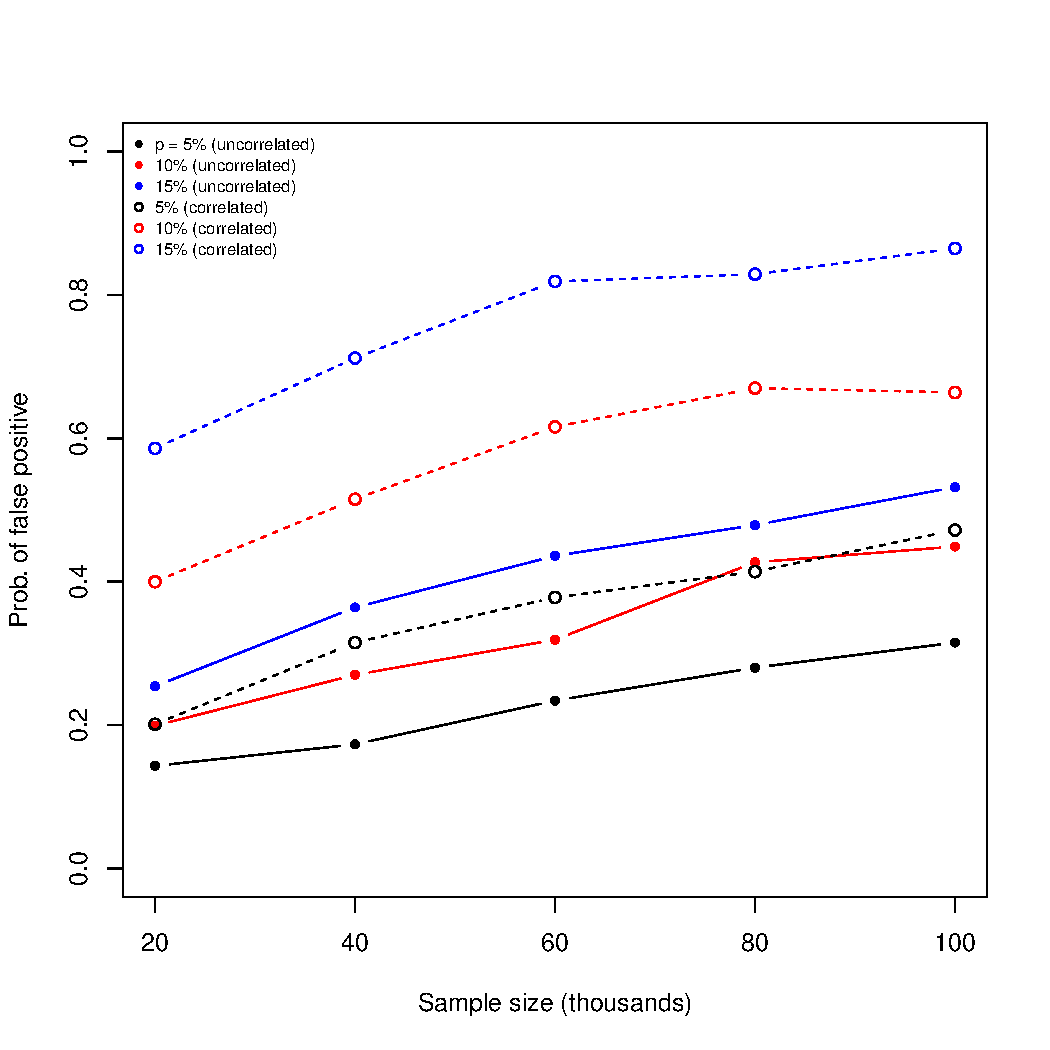
\includegraphics[scale = 0.5]{wcor.pdf}
\caption{ \textbf{. Simulations of Mendelian randomization in the absence of a causal relationship between a trait and a disease.} In addition to the simulations from Figure 1 in the main text, we also performed simulations where the effects of a variant on the trait and on liability to disease were correlated, with a correlation coefficient of 0.4 (see simulation details in the Supplementary Information). Each point is an average over 1,000 simulations.}\label{f_sim}
\end{center}
\end{figure}
\clearpage
\bibliography{../../Bib/bib}
\end{document}